\documentclass[12pt,a4paper]{article}
\usepackage[utf8]{inputenc}
\usepackage[super,sort&compress,numbers]{natbib}
\usepackage{setspace}
\usepackage{geometry}
\usepackage{lineno}
\usepackage{graphicx}
\usepackage{booktabs}
\usepackage{longtable}
\usepackage{amsmath}
\usepackage[hypertexnames=false,hidelinks]{hyperref}
\usepackage{url}
\usepackage{microtype}
\usepackage{float}

\graphicspath{{../manuscript_assets/figures/}{figures/}}

\geometry{margin=3cm}
\doublespacing
\linenumbers

\title{Genetic Tractability of Clinically Relevant Dermatologic Immune Pathway Genes: A Tissue-Aware cis-eQTL Mendelian Randomization Screen}

\author{MU Haoyang\textsuperscript{1} (ORCID: \href{https://orcid.org/0009-0006-1909-2429}{0009-0006-1909-2429}) \\
JIN Shan\textsuperscript{1} (ORCID: \href{https://orcid.org/0000-0002-6268-1759}{0000-0002-6268-1759}) \\
\textsuperscript{1}Department of Dermatology, Yanbian University Hospital, \\
Yanji 133000, China}
\date{}

\begin{document}
\maketitle

\noindent\textbf{Correspondence:} JIN Shan \\
Department of Dermatology, Yanbian University Hospital, Yanji 133000, China \\
Email: 15526770985@163.com

\noindent\textbf{Background:} Human genetics can prioritize therapeutic mechanisms, but clinically validated pathways may be untestable when strong tissue-relevant instruments are absent. We quantified cis-eQTL coverage and screened 19 dermatologic immune pathway genes against four inflammatory skin-disease outcomes.

\noindent\textbf{Methods:} Using GTEx v8 significant-pair files, we selected one lead cis-eQTL per gene--tissue cell in sun-exposed skin, non-sun-exposed skin, and whole blood. Primary instruments required \textit{p} $<5\times10^{-8}$ and F $>10$; relaxed instruments (\textit{p} $<10^{-5}$) were analyzed separately. Single-variant Wald ratios for FinnGen R13 psoriasis, dermatitis and eczema, vitiligo, and alopecia areata were FDR-corrected within each testing family. TYK2 signals underwent external association lookup and Bayesian colocalization.

\noindent\textbf{Results:} Primary instruments were available for 18 of 57 cells (31.6\%); one PDE4A whole-blood variant was absent from all outcomes, leaving 68 primary tests. Three FDR-significant results linked higher genetically proxied TYK2 expression to lower psoriasis risk in sun-exposed skin (OR 0.454, 95\% CI 0.371--0.557), non-sun-exposed skin (OR 0.604, 95\% CI 0.510--0.716), and whole blood (OR 0.507, 95\% CI 0.403--0.637). These three tissue estimates used two variants because rs280497 was shared by non-sun-exposed skin and whole blood. All 23 exact-variant estimates across eight external GWAS records were protective. Colocalization supported a shared TYK2--psoriasis signal in sun-exposed skin (PP.H4 0.825) and whole blood (PP.H4 0.782), but not non-sun-exposed skin (PP.H4 0.220). Relaxed-threshold coverage reached 23 of 57 cells; the PDE4A--psoriasis locus-level analysis was non-supportive (PP.H4 0.108), but the MR SNP was absent from the colocalization rows.

\noindent\textbf{Conclusion:} The screen recovered the established TYK2 psoriasis locus while showing that instrument scarcity constrains dermatologic drug-target MR. Transcript direction should not be equated with pharmacologic inhibition, absence of an instrument is not evidence against a target, and the PDE4A result remains exploratory.

\noindent\textbf{Keywords:} Mendelian randomization, cis-eQTL, psoriasis, TYK2, colocalization, GTEx
\section*{Introduction}

Psoriasis has a complex genetic architecture involving innate and adaptive immune pathways.\textsuperscript{\cite{tsoi2012psoriasis}} The present screen also included dermatitis and eczema, vitiligo, and alopecia areata outcomes to examine genetic tractability across distinct dermatologic phenotypes. Biologics and small molecules directed at the IL-17, IL-23, TNF, JAK, and TYK2 pathways have transformed dermatologic care, but response heterogeneity and failed development programs continue to motivate better target-validation strategies. The selective TYK2 inhibitor deucravacitinib is now an established treatment for moderate-to-severe plaque psoriasis.\textsuperscript{\cite{armstrong2023deucravacitinib}}

Drug-target Mendelian randomization (MR) uses germline variants near a gene to proxy perturbation of a therapeutic mechanism. Targets supported by human genetics are more likely to progress successfully through clinical development, although the validity of any individual MR estimate depends on instrument relevance, exclusion restriction, and appropriate handling of linkage disequilibrium (LD).\textsuperscript{\cite{nelson2015genetic,king2019drugtargets,schmidt2020drugtarget,burgess2023drugdiscovery}} Cis-expression quantitative trait loci (cis-eQTLs) provide one route to instrument gene expression, but regulatory effects are tissue-specific. GTEx therefore offers a useful framework for comparing skin and blood, tissues that capture different components of inflammatory skin disease biology.\textsuperscript{\cite{gtex2020,ongen2017causaltissues}}

A practical limitation is often overlooked: many clinically important genes do not have a sufficiently strong cis-eQTL in the tissue being studied. In that setting, a target is untestable rather than genetically unsupported. Conflating the absence of an instrument with evidence of no effect can distort target prioritization.\textsuperscript{\cite{gill2024pitfalls,sanderson2022mr}} This concern is especially relevant to cytokines, receptors, intracellular kinases, and barrier genes whose expression may be cell-state-specific or poorly captured in bulk tissue.

The TYK2 locus provides a useful positive-control benchmark. TYK2 coding variation, including P1104A, is associated with autoimmune protection, and pharmacologic TYK2 inhibition is effective in psoriasis.\textsuperscript{\cite{steri2025tyk2,armstrong2023deucravacitinib}} Previous MR and colocalization studies have also implicated TYK2 in psoriasis.\textsuperscript{\cite{guo2024tyk2,yuan2023tyk2}} Recovery of a TYK2 psoriasis signal can therefore test whether a tissue-aware pipeline detects an established locus. Importantly, however, the direction of an expression-based instrument cannot automatically be equated with the direction of kinase inhibition because a locus may contain coding and regulatory effects with different molecular consequences.

We therefore screened a curated panel of 19 clinically relevant dermatologic immune pathway genes across sun-exposed skin, non-sun-exposed skin, and whole blood. The panel deliberately included direct drug targets, target-family members, pathway genes, and disease-relevant controls rather than 19 direct targets of marketed drugs. We treated instrument availability as a primary result, performed a threshold-defined genome-wide-significant analysis and a separately corrected relaxed-threshold analysis, and evaluated TYK2 with locus inspection, external association data, and tissue-resolved colocalization. The study design is shown in Figure~1.

\section*{Material and Methods}

\subsection*{Study Design}

This two-sample MR study was reported with reference to STROBE-MR guidance.\textsuperscript{\cite{skrivankova2021strobemr,burgess2021mr}} The workflow comprised target-panel definition, tissue-specific cis-eQTL instrument selection, harmonization with four FinnGen outcomes, single-SNP MR with multiple-testing correction, and focused validation of the established TYK2 signal (Figure~1). All inputs were publicly available, de-identified summary statistics. The study was not prospectively registered, and no analysis protocol was deposited before the analyses were performed.

\subsection*{Target Gene Panel}

We curated 19 genes spanning clinically relevant dermatologic immune pathways: \textit{JAK1}, \textit{JAK2}, \textit{JAK3}, \textit{TYK2}, \textit{IL4R}, \textit{IL13}, \textit{IL17A}, \textit{IL17RA}, \textit{IL23A}, \textit{IL23R}, \textit{TNF}, \textit{PDE4A}, \textit{PDE4B}, \textit{PDE4C}, \textit{PDE4D}, \textit{IL36RN}, \textit{TSLP}, \textit{FLG}, and \textit{CARD14}. The panel included direct drug targets, members of drug-target families, pathway genes, and the barrier or disease-relevant controls \textit{FLG} and \textit{CARD14}; it was not intended to imply that every encoded protein is directly targeted by an approved dermatologic therapy. Gene symbols were mapped to GENCODE v26 Ensembl identifiers. Because the study was not preregistered and the panel was not derived from a systematic review, inference is limited to this curated set rather than all dermatologic drug targets.

\subsection*{Exposure Data and Instrument Selection}

GTEx v8 significant cis-eQTL variant--gene pair files were used for skin sun-exposed lower leg, skin not sun-exposed suprapubic, and whole blood.\textsuperscript{\cite{gtex2020}} These files contain GTEx-significant pairs rather than complete all-pairs cis summary statistics. Instrument-availability estimates are therefore conditional on the released significant-pair sets and may undercount nominal cis associations that were not included in those files. For the primary analysis, a candidate instrument required an eQTL \textit{p}-value $<5\times10^{-8}$ and an approximate F-statistic $>10$, where $F=(\beta_{\mathrm{exposure}}/SE_{\mathrm{exposure}})^2$.\textsuperscript{\cite{burgess2011weak}} Within each gene--tissue cell, the variant with the smallest eQTL \textit{p}-value was retained; exact ties were resolved by ascending GTEx variant identifier.

No matched genotype LD reference panel was available. We therefore did not claim LD clumping and did not construct multi-SNP instruments. Each analysis used one deterministic lead cis-eQTL, an approach that avoids treating correlated variants as independent but cannot by itself exclude LD confounding by a distinct causal variant.\textsuperscript{\cite{gkatzionis2022cismr,lin2024cismr}} A separate exploratory analysis considered cells with no primary instrument but an eQTL \textit{p}-value $<10^{-5}$ and F $>10$. These relaxed-threshold tests were analyzed and corrected separately from the primary family.

\subsection*{Outcome Data}

Outcome summary statistics were obtained from FinnGen release R13.\textsuperscript{\cite{kurki2023finngen}} The endpoints were psoriasis (L12\_PSORIASIS; 13,309 cases and 481,187 controls), dermatitis and eczema (L12\_DERMATITISECZEMA; 72,371 cases and 427,815 controls), vitiligo (L12\_VITILIGO; 421 cases and 462,830 controls), and alopecia areata (L12\_ALOPECAREATA; 994 cases and 474,896 controls). FinnGen beta coefficients were treated as per-alternate-allele log odds ratios. GTEx and FinnGen are distinct resources, so participant overlap is not expected, although individual-level overlap could not be checked from summary data. The low case counts for vitiligo and alopecia areata were considered when interpreting null estimates; no formal power percentages were reported because a validated exposure R-squared and binary-outcome power model were not available.

\subsection*{Instrumental-Variable Assumptions}

The analysis relied on the three core instrumental-variable assumptions. Relevance was addressed by restricting instruments to cis-eQTLs that met the specified \textit{p}-value and F-statistic thresholds. Independence from exposure--outcome confounders could not be tested directly with summary statistics; cis restriction and the covariate-adjusted source GWAS reduce but do not eliminate this concern. The exclusion-restriction assumption---that the variant influences disease only through the measured gene-expression exposure---also cannot be verified for a single cis variant. Tissue comparison, locus inspection, and colocalization were therefore used as supporting assessments, but none can exclude horizontal pleiotropy or a distinct causal variant in linkage disequilibrium.

\subsection*{Mendelian Randomization and Statistical Analysis}

GTEx and FinnGen variants were matched by GRCh38 chromosome, position, reference allele, and alternate allele. Outcome effects were sign-flipped when the reference and alternate alleles were reversed. Variants absent from an outcome file were recorded as unmatched and were not imputed or replaced with proxies in the primary analysis. The analyses used the covariate-adjusted summary statistics released by each consortium; individual-level covariates were not refitted, and identical covariate sets across resources could not be guaranteed. For each matched variant, the Wald ratio was

\begin{equation}
\hat{\beta}_{\mathrm{MR}} =
\frac{\hat{\beta}_{\mathrm{outcome}}}{\hat{\beta}_{\mathrm{exposure}}}.
\label{eq:wald}
\end{equation}

The primary standard error followed the conventional first-order single-SNP approximation used by TwoSampleMR:

\begin{equation}
SE_{\mathrm{primary}} =
\left|\frac{SE_{\mathrm{outcome}}}{\hat{\beta}_{\mathrm{exposure}}}\right|.
\label{eq:se-primary}
\end{equation}

As a robustness analysis, we also calculated the full delta-method standard error including uncertainty in the SNP--exposure association:

\begin{equation}
SE_{\mathrm{delta}} =
\sqrt{\frac{SE_{\mathrm{outcome}}^2}{\hat{\beta}_{\mathrm{exposure}}^2}
+ \frac{\hat{\beta}_{\mathrm{outcome}}^2SE_{\mathrm{exposure}}^2}
{\hat{\beta}_{\mathrm{exposure}}^4}}.
\label{eq:se-delta}
\end{equation}

Effects were exponentiated to odds ratios (ORs) with 95\% confidence intervals. Benjamini--Hochberg FDR correction was applied across all primary tests and, separately, across all relaxed-threshold tests.\textsuperscript{\cite{benjamini1995fdr}} FDR $<0.05$ was considered significant. Nominal \textit{p} $<0.05$ with FDR $\geq0.05$ was reported descriptively. Final verification used R 4.6.0 with TwoSampleMR 0.7.6, coloc 5.2.3, data.table 1.18.4, dplyr 1.2.1, yaml 2.3.12, readr 2.2.0, jsonlite 2.0.0, and ggplot2 4.0.3.\textsuperscript{\cite{hemani2018twosamplemr}} The optional OpenGWAS refresh used ieugwasr 1.1.0. The independent raw-data audit used Python 3.10.4 with pandas 2.3.3 and NumPy 2.2.6.

\subsection*{TYK2 Validation and External Association Lookup}

Because all primary FDR-significant rows represented TYK2, validation focused on this established positive-control locus. We verified each instrument's rank among GTEx significant TYK2 cis-eQTLs and ranked variants within the FinnGen psoriasis locus ($\pm500$ kb). We then extracted available non-FinnGen psoriasis or psoriatic-arthritis association records through OpenGWAS and recomputed tissue-specific Wald ratios using the corresponding GTEx exposure estimates. Only exact requested-variant matches were retained; one unresolved proxy result was excluded because the local export did not preserve the proxy SNP or its LD estimate. External records were treated as directional concordance rather than as statistically independent replication because overlap among contributing studies could not be excluded.

\subsection*{Colocalization Analysis}

GTEx significant-pair files do not contain complete locus-wide data, so full cis-eQTL summary statistics were obtained from three eQTL Catalogue GTEx v8 datasets: QTD000316 for sun-exposed skin, QTD000311 for non-sun-exposed skin, and QTD000356 for whole blood.\textsuperscript{\cite{kerimov2021eqtlcatalogue}} FinnGen psoriasis and eQTL data were aligned within a 1 Mb TYK2 window. Bayesian colocalization used the \textit{coloc} package with priors $p_1=10^{-4}$, $p_2=10^{-4}$, and $p_{12}=10^{-5}$.\textsuperscript{\cite{giambartolomei2014coloc}} The eQTL datasets were modeled as quantitative traits with sample sizes 602, 517, and 670 for QTD000316, QTD000311, and QTD000356, respectively, and with $sdY=1$; FinnGen psoriasis was modeled as a case--control trait with 13,309 cases and 481,187 controls. The \textit{coloc.abf} model assumes at most one causal variant per trait within the analyzed region; unmodeled allelic heterogeneity may affect posterior probabilities. PP.H4 represents a shared causal variant; PP.H3 represents two distinct causal variants; and PP.H2 represents association with the GWAS trait only. PP.H4 $\geq0.80$ was considered strong support and PP.H4 $\geq0.50$ supportive evidence.\textsuperscript{\cite{zuber2022coloc}} For TYK2 tissues with PP.H4 $\geq0.50$, \textit{coloc::sensitivity} varied $p_{12}$ across the evaluated range from $10^{-8}$ to $10^{-4}$ and assessed the rule PP.H4 $\geq0.50$; plots were not generated for base analyses below that support threshold. The relaxed-threshold PDE4A psoriasis signal was evaluated with the same locus-level framework but remained outside the primary analysis. The selected PDE4A MR instrument itself was absent from the eQTL Catalogue rows used for colocalization, so this analysis did not directly test whether the MR variant shared the psoriasis causal signal.

\subsection*{Reproducibility Audit}

All three GTEx files and all four FinnGen files were independently reread from the local compressed raw data. This audit regenerated instrument selection, allele harmonization, Wald estimates, confidence intervals, and both FDR families. The 68 primary results matched the saved R output with maximum absolute differences below $10^{-14}$ for beta, standard error, \textit{p}-value, and FDR. Reverse MR and Steiger directionality were not reported because the available GTEx files contain selected significant pairs rather than all-variant outcome summary statistics, and the stored \texttt{ma\_samples} field is not the tissue sample size required for a valid directionality calculation.

\section*{Results}

\subsection*{Instrument Availability}

The panel contained 57 gene--tissue cells. At the primary threshold, 18 cells (31.6\%) across nine genes had a lead cis-eQTL: five in sun-exposed skin, seven in non-sun-exposed skin, and six in whole blood (Figure~3; Table~1; Supplementary Table S2). Primary-instrument F-statistics ranged from 33.6 to 447.9. The PDE4A whole-blood lead variant was absent from all four FinnGen outcome files, leaving 17 analyzable cells across eight genes.

The relaxed threshold added five cells: IL36RN in sun-exposed skin, PDE4A in sun-exposed skin, PDE4B in both skin tissues, and PDE4C in sun-exposed skin. Conditional coverage within the three GTEx significant-pair files was therefore 23 of 57 cells (40.4\%) across 11 genes. Eight genes had no eligible row in any tissue even at the relaxed threshold: \textit{JAK2}, \textit{JAK3}, \textit{IL13}, \textit{IL17A}, \textit{IL23A}, \textit{IL23R}, \textit{TNF}, and \textit{PDE4D}. These genes are untestable in the present significant-pair design; this is not evidence of no therapeutic effect or proof that no nominal cis association exists in complete all-pairs data.

\subsection*{Primary MR Results}

The 17 analyzable cells generated 68 primary Wald-ratio tests (Figure~2; Supplementary Table S3). Three rows reached FDR $<0.05$, all for TYK2 and psoriasis. Higher genetically proxied TYK2 expression was associated with lower psoriasis risk in sun-exposed skin (OR 0.454, 95\% CI 0.371--0.557; \textit{p} $=2.50\times10^{-14}$; FDR $=1.70\times10^{-12}$), non-sun-exposed skin (OR 0.604, 95\% CI 0.510--0.716; \textit{p} $=5.91\times10^{-9}$; FDR $=1.34\times10^{-7}$), and whole blood (OR 0.507, 95\% CI 0.403--0.637; \textit{p} $=5.91\times10^{-9}$; FDR $=1.34\times10^{-7}$).

Two additional estimates were nominally associated but did not survive FDR correction: CARD14 expression in whole blood with psoriasis (OR 1.106, 95\% CI 1.031--1.187; \textit{p} $=0.00519$; FDR $=0.0883$) and JAK1 expression in whole blood with dermatitis and eczema (OR 0.870, 95\% CI 0.765--0.991; \textit{p} $=0.0356$; FDR $=0.484$). No vitiligo or alopecia areata result was FDR-significant.

The full delta-method sensitivity analysis retained all three TYK2 signals, with FDR values from $3.10\times10^{-5}$ to $7.94\times10^{-5}$, and did not change any result category (Supplementary Table S8).

\subsection*{TYK2 Locus and External Association Lookup}

The non-sun-exposed skin and whole-blood estimates used rs280497, whereas the sun-exposed skin estimate used rs35251378. Each was the rank-1 TYK2 cis-eQTL in its respective GTEx tissue (Supplementary Table S5). Within the FinnGen psoriasis locus, rs34536443 was the lead variant; rs35251378 ranked fourth and rs280497 ranked eleventh. These ranks establish that the MR instruments lie within the associated TYK2 locus but do not by themselves establish that the variants are interchangeable or in the same LD block.

Eight non-FinnGen records were obtained from OpenGWAS, covering psoriasis, psoriasis vulgaris, self-reported psoriasis, and psoriatic arthritis. Across these records, 23 exact-variant tissue-specific Wald-ratio estimates were available, all with a protective direction (Supplementary Table S6 and Supplementary Figure S1). One additional proxy-supported export was excluded because the proxy SNP and LD estimate were not retained locally. This concordance provides external directional support but does not constitute independent replication: the rows reuse two variants across three tissues, and contributing GWAS samples may overlap.

\subsection*{Tissue-Resolved Colocalization}

TYK2 colocalization was tissue-dependent (Figure~4; Supplementary Table S7). Sun-exposed skin showed strong support for a shared signal (2,474 overlapping variants; PP.H4 0.825). Whole blood showed supportive evidence (2,494 variants; PP.H4 0.782). Non-sun-exposed skin did not support colocalization (1,969 variants; PP.H4 0.220), with posterior probability concentrated on the GWAS-only model (PP.H2 0.653). Prior-sensitivity checks for sun-exposed skin and whole blood retained PP.H4 $\geq0.50$ at the analysis value $p_{12}=10^{-5}$ and at larger evaluated $p_{12}$ values, but fell below 0.50 at sufficiently smaller evaluated $p_{12}$ values; the support is therefore prior-dependent. A plot was not generated for non-sun-exposed skin because its base PP.H4 was below 0.50. Thus, the TYK2 locus was recovered in all three MR analyses, but shared-variant support was strongest in sun-exposed skin and whole blood.

\subsection*{Separate Relaxed-Threshold Analysis}

The five relaxed-only cells generated 20 tests corrected as a separate family (Supplementary Table S4). PDE4A expression in sun-exposed skin was associated with psoriasis (OR 2.832, 95\% CI 1.883--4.257; \textit{p} $=5.65\times10^{-7}$; relaxed-family FDR $=1.13\times10^{-5}$). Its exposure instrument was below genome-wide significance (\textit{p} $=3.65\times10^{-6}$; F $=21.9$), and the locus-level colocalization analysis did not support a shared psoriasis causal variant (PP.H4 0.108; PP.H2 0.753). The selected MR instrument was absent from the PDE4A eQTL Catalogue rows used for colocalization, so this analysis did not directly test that variant and should be regarded as non-supportive rather than definitive. This result is therefore exploratory and was not promoted to the primary findings. JAK2 did not meet either the primary or relaxed instrument threshold and was not analyzed in the threshold-defined MR families.

\section*{Discussion}

This tissue-aware screen produced two main findings. First, the threshold-defined primary analysis recovered TYK2 as the only FDR-significant gene, with psoriasis associations in both skin tissues and whole blood. Second, strict instrument coverage was limited: only 18 of 57 gene--tissue cells had a genome-wide-significant cis-eQTL, and only 17 cells could be matched to the four FinnGen outcomes. The study therefore functions more convincingly as an assessment of genetic tractability within the curated panel and an established-locus positive control than as a discovery screen for new drug targets.

The TYK2 result requires careful directional interpretation. The eQTL alleles associated with higher measured TYK2 transcript were associated with lower psoriasis risk. This should not be translated into a claim that increasing TYK2 expression is therapeutic or that the eQTL directly mimics pharmacologic inhibition. The TYK2 locus contains coding and regulatory variation, transcript abundance may not proxy kinase activity, and bulk-tissue eQTL effects may differ across cell types or activation states. The MR odds ratios are scaled to genetically proxied transcript differences and are not estimates of deucravacitinib or any other drug effect. The value of TYK2 as a positive control is therefore the recovery and validation of an established psoriasis locus, not a simple match between the sign of the transcript estimate and the direction of deucravacitinib treatment.\textsuperscript{\cite{steri2025tyk2,armstrong2023deucravacitinib}}

The colocalization results refine that interpretation. Strong shared-variant support in sun-exposed skin and supportive evidence in whole blood strengthen the case that the expression and psoriasis signals overlap in those datasets. In non-sun-exposed skin, PP.H2 exceeded PP.H4, so the MR association alone is insufficient to infer shared causality. Colocalization itself does not prove that altered TYK2 expression is the mediating molecular mechanism, particularly in a locus with coding variation, but it reduces concern that the two associations arise from completely distinct variants in sun-exposed skin and whole blood.\textsuperscript{\cite{giambartolomei2014coloc,zuber2022coloc}}

Instrument scarcity was not confined to one pathway. At the primary threshold, only nine of 19 genes were represented in at least one tissue. A relaxed threshold added IL36RN and PDE4B, raising gene-level coverage to 11 of 19, but eight genes remained uninstrumented. Several are clinically important, including TNF, IL17A, IL23R, and JAK3. Their absence from the MR results reflects the limitations of bulk-tissue expression resources, the selected thresholds, and the use of GTEx significant-pair rather than complete all-pairs files; it is not evidence against their established therapeutic relevance.\textsuperscript{\cite{gill2024pitfalls}} Future work may improve coverage with larger skin eQTL studies, cell-type-specific QTLs, coding variants, or rigorously curated protein QTL resources.\textsuperscript{\cite{sun2023plasma,ferkingstad2021proteome,trajanoska2023target}}

The separate PDE4A result illustrates why threshold provenance and colocalization matter. Its association was statistically strong within the 20-test relaxed family, but the exposure eQTL did not meet the primary genome-wide-significance criterion and locus-level PP.H4 was only 0.108. The selected MR instrument was absent from the eQTL Catalogue rows used for colocalization, so the analysis did not directly test that variant and is non-supportive rather than definitive. The result may reflect instrument-selection uncertainty, LD, or locus architecture and should not be presented as genetic validation of PDE4A inhibition. JAK2 was not testable because no eligible row met either threshold; accordingly, no JAK2 estimate is reported.

\subsection*{Clinical Implications for Target Selection}

The findings define three clinically distinct evidence states. First, recovery of an established locus with shared-variant support, as for TYK2 in sun-exposed skin and whole blood, justifies further mechanistic study but does not by itself establish the direction or magnitude of a pharmacologic intervention. Second, absence of an eligible instrument, as for TNF, IL17A, IL23R, and JAK3, means that the target is not testable in this dataset and should be judged using other evidence streams, including disease-tissue biology, functional studies, and clinical trials. Third, an association based on a relaxed instrument without colocalization support, as for PDE4A, should remain a low-confidence hypothesis until replicated with stronger instruments, fine-mapping, or orthogonal molecular data. This three-state interpretation is more useful for clinical target selection than a binary supported-versus-unsupported label.

This study has several strengths. All seven compressed source files were reread, the 68 primary estimates were independently reproduced to numerical precision, primary and relaxed hypotheses were corrected separately, and every reported MR row can be traced to its exposure and outcome beta, standard error, and allele orientation. Reporting the 57-cell availability matrix also makes the denominator of the screen explicit. Finally, tissue-resolved colocalization prevented a uniform interpretation of three superficially concordant TYK2 MR estimates.

The limitations are substantial. Each estimate used one variant, so MR-Egger, weighted median, heterogeneity testing, and MR-PRESSO were not possible. No external LD reference was available, and lead-variant selection is not a substitute for LD clumping or correlated-instrument cis-MR.\textsuperscript{\cite{gkatzionis2022cismr,lin2024cismr}} A single-SNP Wald ratio cannot exclude horizontal pleiotropy, whose direction is not predictable from the available data. The three TYK2 tissue rows rely on only two distinct variants and are partly non-independent. The significant-pair GTEx files do not provide a complete inventory of nominal cis associations, so the relaxed-threshold coverage is conditional and may be underestimated. The single-causal-variant assumption of \textit{coloc.abf} may be violated by allelic heterogeneity, which could affect the reported posterior probabilities. The eQTL colocalization inputs also used $sdY=1$, an assumed unit phenotypic standard deviation whose misspecification could affect Bayes factors and posterior probabilities. Reverse MR and Steiger analyses could not be validly performed with significant-pair-only GTEx files and unverified tissue sample sizes. Formal power percentages were not defensible; the much smaller vitiligo and alopecia areata case counts imply lower precision and warrant caution when interpreting null results. The study was not prospectively registered. GTEx represents mostly healthy bulk tissue, FinnGen is ancestry-specific, and the external GWAS records may overlap. Lifelong genetically proxied expression differences cannot be assumed to represent treatment timing, dose, duration, or expression changes outside the genetically observed range. The target panel also mixes direct targets with pathway and disease genes, so results should be interpreted at the gene and locus level rather than as uniform pharmacologic proxies.

Within these constraints, the data support a narrow conclusion: the pipeline recovers the established TYK2 psoriasis locus, with the strongest shared-variant evidence in sun-exposed skin and whole blood, while current GTEx resources leave most panel gene--tissue cells untestable. Dermatologic drug-target MR studies should therefore report instrument coverage, threshold provenance, and colocalization alongside effect estimates.

\section*{Conclusions}

The threshold-defined primary analysis comprised 68 analyzable tests. TYK2 was the only FDR-significant gene and served as an established psoriasis-locus positive control. Colocalization supported a shared signal in sun-exposed skin and whole blood but not in non-sun-exposed skin. Conditional cis-eQTL coverage within the GTEx significant-pair files was limited to 18 of 57 gene--tissue cells, and only 17 cells could be analyzed against all four outcomes. A relaxed-threshold PDE4A association lacked locus-level colocalization support and remains exploratory. These findings emphasize that instrument scarcity, single-variant uncertainty, and the distinction between transcript effects and pharmacologic modulation must be explicit in dermatologic drug-target MR.

\section*{Abbreviations}

cis-eQTL, cis-expression quantitative trait locus; CI, confidence interval; FDR, false discovery rate; GTEx, Genotype-Tissue Expression; GWAS, genome-wide association study; LD, linkage disequilibrium; MR, Mendelian randomization; OR, odds ratio; PP.H2, posterior probability of association with the GWAS trait only; PP.H3, posterior probability of association with both traits through distinct causal variants; PP.H4, posterior probability of a shared causal variant; SE, standard error; SNP, single nucleotide polymorphism; STROBE-MR, Strengthening the Reporting of Observational Studies in Epidemiology using Mendelian Randomization; TYK2, tyrosine kinase 2.

\section*{Ethics Approval and Informed Consent}

This study used only publicly available, de-identified genome-wide association study and expression quantitative trait locus summary statistics. No new individual-level data were generated or accessed, and no new ethical approval or informed consent was required. The original data sources, including GTEx, FinnGen, OpenGWAS, and the eQTL Catalogue, obtained ethics approvals and participant consent within their respective consortia.

\section*{Consent for Publication}

Not applicable. This study used only de-identified summary-level data and contains no individual patient information, images, or recordings.

\section*{Data Availability}

Public summary statistics analyzed in this study are available from the \href{https://gtexportal.org/home/}{GTEx Portal}, \href{https://r13.finngen.fi/}{FinnGen release R13}, \href{https://gwas.mrcieu.ac.uk/}{OpenGWAS}, and the \href{https://www.ebi.ac.uk/eqtl/}{eQTL Catalogue} datasets QTD000316, QTD000311, and QTD000356. The corrected analysis scripts, the 68-row primary result table with exposure and outcome association fields, the relaxed-threshold results, reproducibility-audit outputs, and curated validation tables are deposited in a versioned public archive at \href{https://github.com/muhaoyang0616/skin_drug_target_mr/releases/tag/v1.0.0}{GitHub release v1.0.0} (archived on Zenodo at \href{https://doi.org/10.5281/zenodo.21331678}{10.5281/zenodo.21331678}). Source code is released under the MIT License, and manuscript source, figures, documentation, and machine-readable result tables are released under the Creative Commons Attribution 4.0 International License; raw GTEx and FinnGen files are not redistributed and remain subject to the terms of their originating resources.

\section*{Funding}

This work received no specific grant from any funding agency in the public, commercial, or not-for-profit sectors; therefore, no funder had any role in study design, analysis, interpretation, manuscript preparation, or the decision to submit.

\section*{Competing Interests}

The authors declare that they have no competing financial or non-financial interests related to the content of this article.

\section*{Authors' Contributions}

MH conceived and designed the study, performed the data analysis, interpreted the results, and drafted the manuscript. JS supervised the study, contributed to data interpretation, and critically revised the manuscript. Both authors read and approved the final version and agree to be accountable for the content of this work.

\section*{Acknowledgments}

The authors acknowledge the GTEx Consortium, FinnGen project, OpenGWAS database, and eQTL Catalogue for making their summary statistics publicly available. We thank the participants and investigators of these consortia for their contributions to open science.

\section*{AI-Assisted Technologies Disclosure}

OpenAI Codex was used solely for language editing, cross-document consistency checking, and formatting. It was not used to generate or alter research data, statistical analyses or results, or scientific conclusions. All AI-assisted edits were reviewed and approved by the authors, who take full responsibility for the final manuscript.


\clearpage
\section*{Tables}

\begin{table}[H]
\centering
\caption{Cis-eQTL instrument availability across 19 genes and three GTEx v8 tissues.}
\label{tab:1}
\footnotesize
\resizebox{\textwidth}{!}{%
\begin{tabular}{lccccc}
\toprule
\textbf{Gene} & \textbf{Sun-exposed skin} & \textbf{Non-sun-exposed skin} & \textbf{Whole blood} & \textbf{Primary tissues} & \textbf{Any tissues} \\
\midrule
\textit{JAK1}    & -- & P  & P  & 2 & 2 \\
\textit{JAK2}    & -- & -- & -- & 0 & 0 \\
\textit{JAK3}    & -- & -- & -- & 0 & 0 \\
\textit{TYK2}    & P  & P  & P  & 3 & 3 \\
\textit{IL4R}    & -- & -- & P  & 1 & 1 \\
\textit{IL13}    & -- & -- & -- & 0 & 0 \\
\textit{IL17A}   & -- & -- & -- & 0 & 0 \\
\textit{IL17RA}  & P  & P  & P  & 3 & 3 \\
\textit{IL23A}   & -- & -- & -- & 0 & 0 \\
\textit{IL23R}   & -- & -- & -- & 0 & 0 \\
\textit{TNF}     & -- & -- & -- & 0 & 0 \\
\textit{PDE4A}   & E  & -- & P\textsuperscript{a} & 1 & 2 \\
\textit{PDE4B}   & E  & E  & -- & 0 & 2 \\
\textit{PDE4C}   & E  & P  & -- & 1 & 2 \\
\textit{PDE4D}   & -- & -- & -- & 0 & 0 \\
\textit{IL36RN}  & E  & -- & -- & 0 & 1 \\
\textit{TSLP}    & P  & P  & -- & 2 & 2 \\
\textit{FLG}     & P  & P  & -- & 2 & 2 \\
\textit{CARD14}  & P  & P  & P  & 3 & 3 \\
\midrule
\textbf{Total cells} & \textbf{5 P + 4 E} & \textbf{7 P + 1 E} & \textbf{6 P} & \textbf{18 / 57} & \textbf{23 / 57} \\
\bottomrule
\end{tabular}
}

\vspace{4pt}
\noindent\footnotesize P, primary instrument (\textit{p} $<5\times10^{-8}$ and F $>10$); E, exploratory relaxed-only instrument (\textit{p} $<10^{-5}$ and F $>10$ in a cell without a primary instrument); --, no eligible row in the analyzed GTEx significant-pair file at either threshold. \textsuperscript{a}The PDE4A whole-blood primary variant was absent from all four FinnGen outcome files and did not generate an MR estimate. Variant-level details are provided in Supplementary Table S2.
\end{table}
\clearpage


\bibliographystyle{unsrt}
\bibliography{refs}

\clearpage
\section*{Figure Legends}

\begin{figure}[H]
\centering
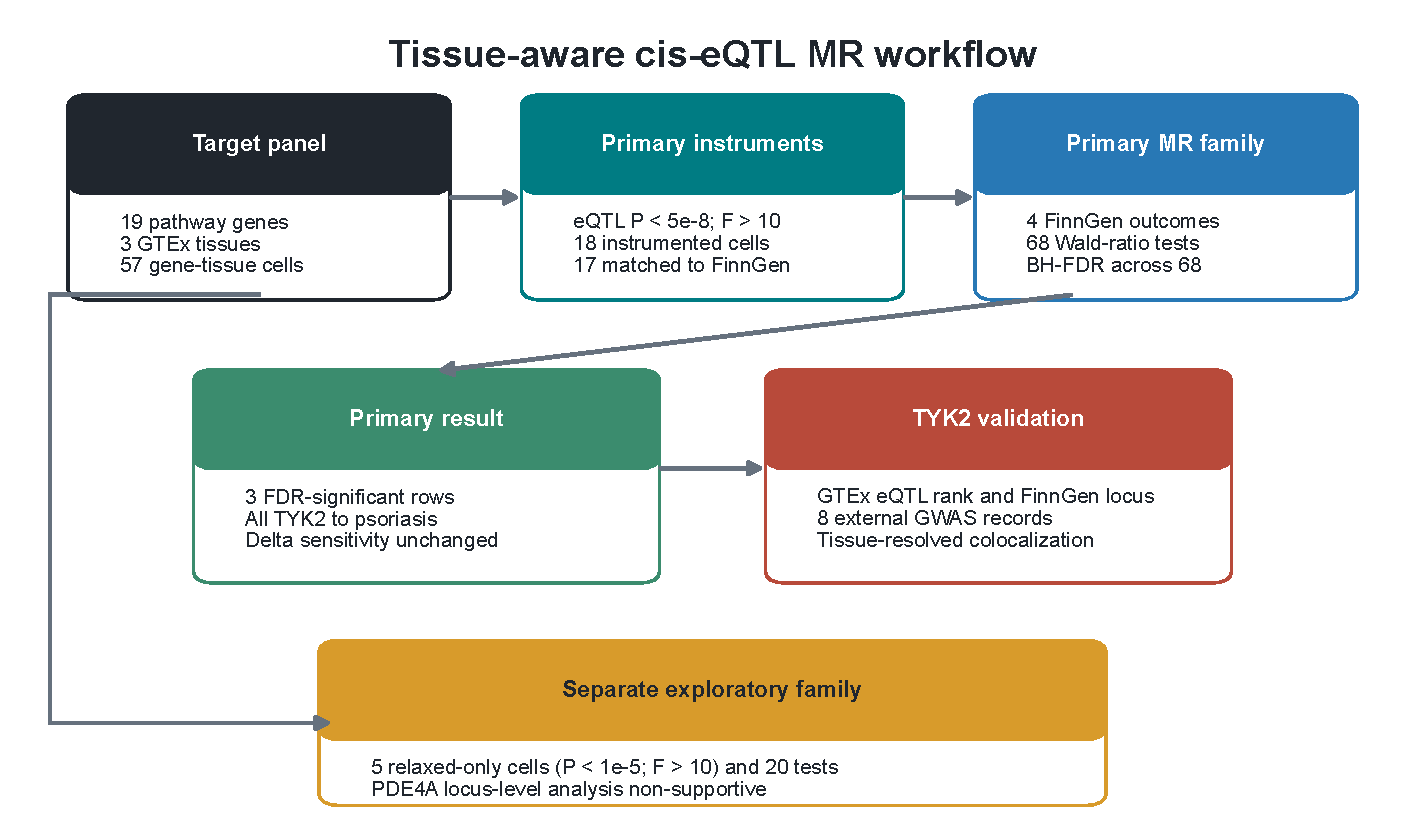
\includegraphics[width=\textwidth,height=0.56\textheight,keepaspectratio]{figure1_study_design_flowchart.pdf}
\caption{Study design. Nineteen curated dermatologic immune pathway genes formed 57 gene--tissue cells across two skin tissues and whole blood. Eighteen cells met the primary instrument threshold; one PDE4A whole-blood variant was absent from FinnGen, leaving 17 cells and 68 primary tests. A separate relaxed-threshold family contained five additional cells and 20 tests. Primary FDR-significant TYK2 results underwent locus, external-association, and colocalization validation.}
\label{fig:1}
\end{figure}

\clearpage
\begin{figure}[H]
\centering
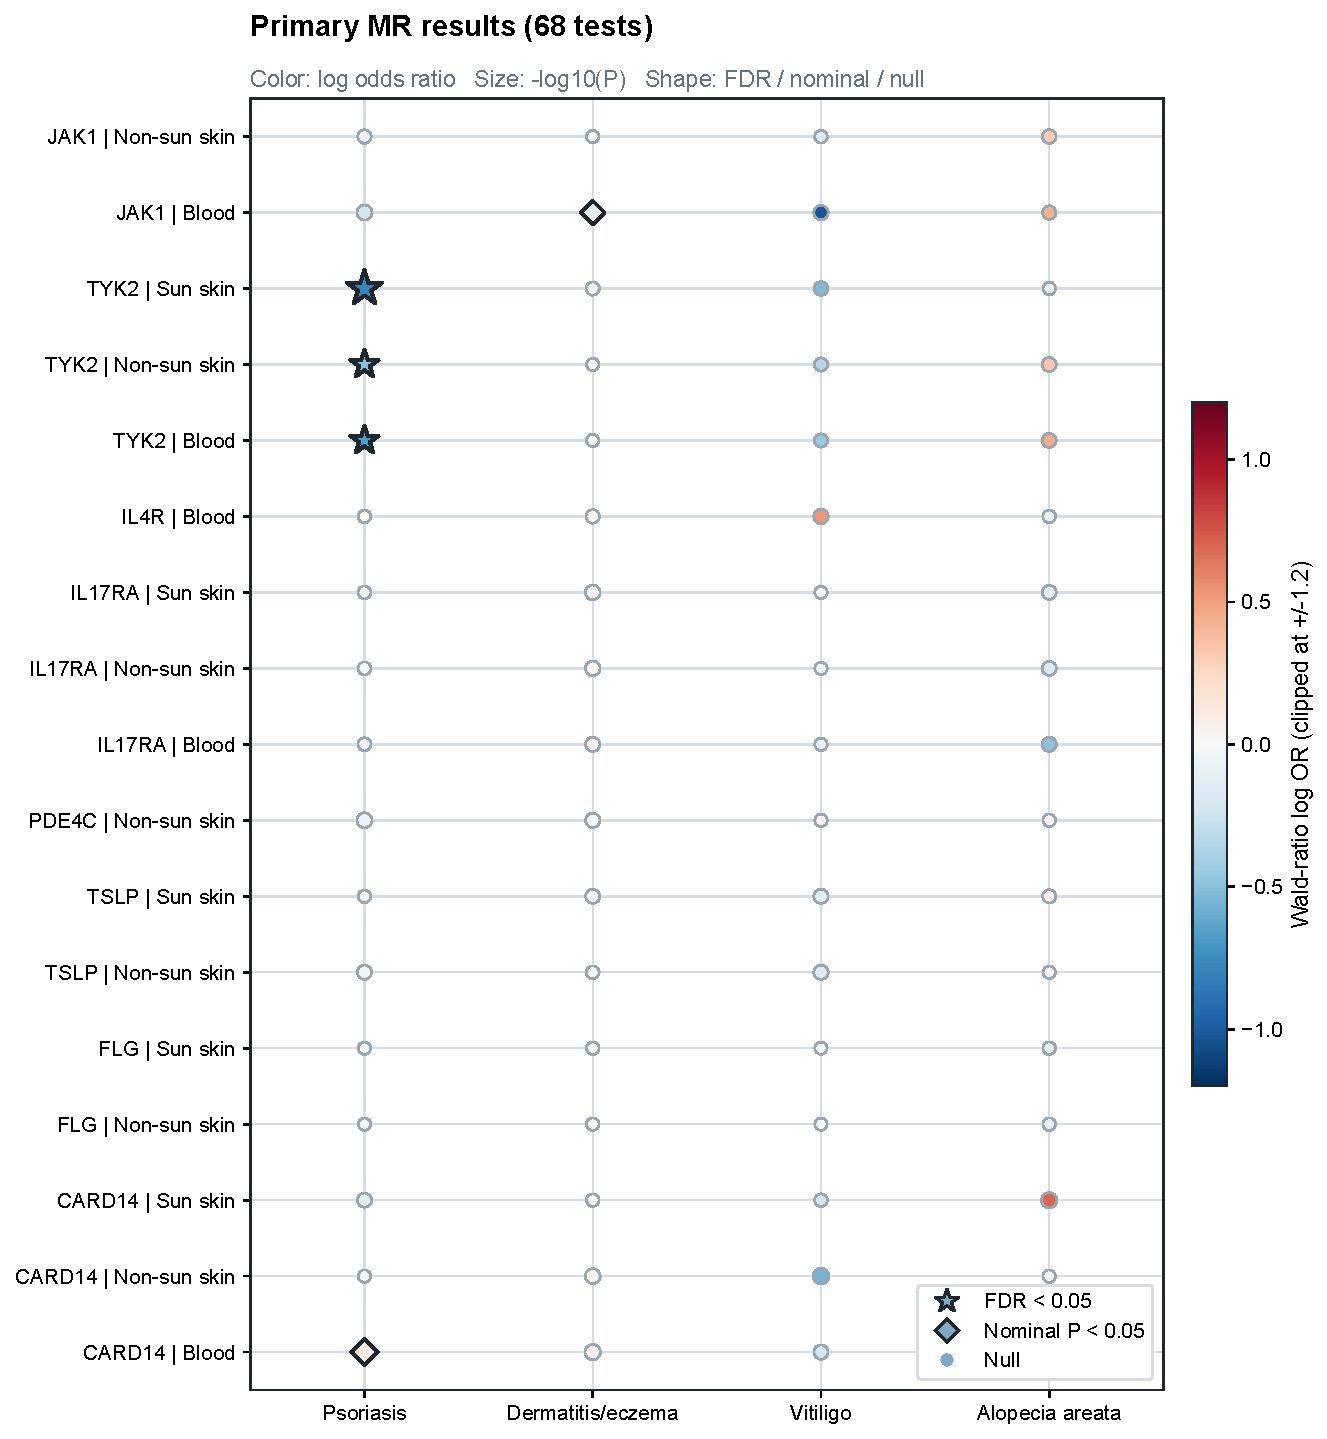
\includegraphics[width=\textwidth,height=0.68\textheight,keepaspectratio]{figure2_mr_results.pdf}
\caption{Primary Mendelian randomization results. The 68 gene--tissue--outcome tests are displayed as a bubble matrix. Color encodes the Wald-ratio log odds ratio (clipped at $\pm1.2$ for display), marker area encodes $-\log_{10}(p)$, and marker shape distinguishes FDR-significant, nominal, and null results. The three TYK2--psoriasis estimates were FDR-significant; CARD14--psoriasis and JAK1--dermatitis/eczema were nominally associated but did not survive FDR correction.}
\label{fig:2}
\end{figure}

\clearpage
\begin{figure}[H]
\centering
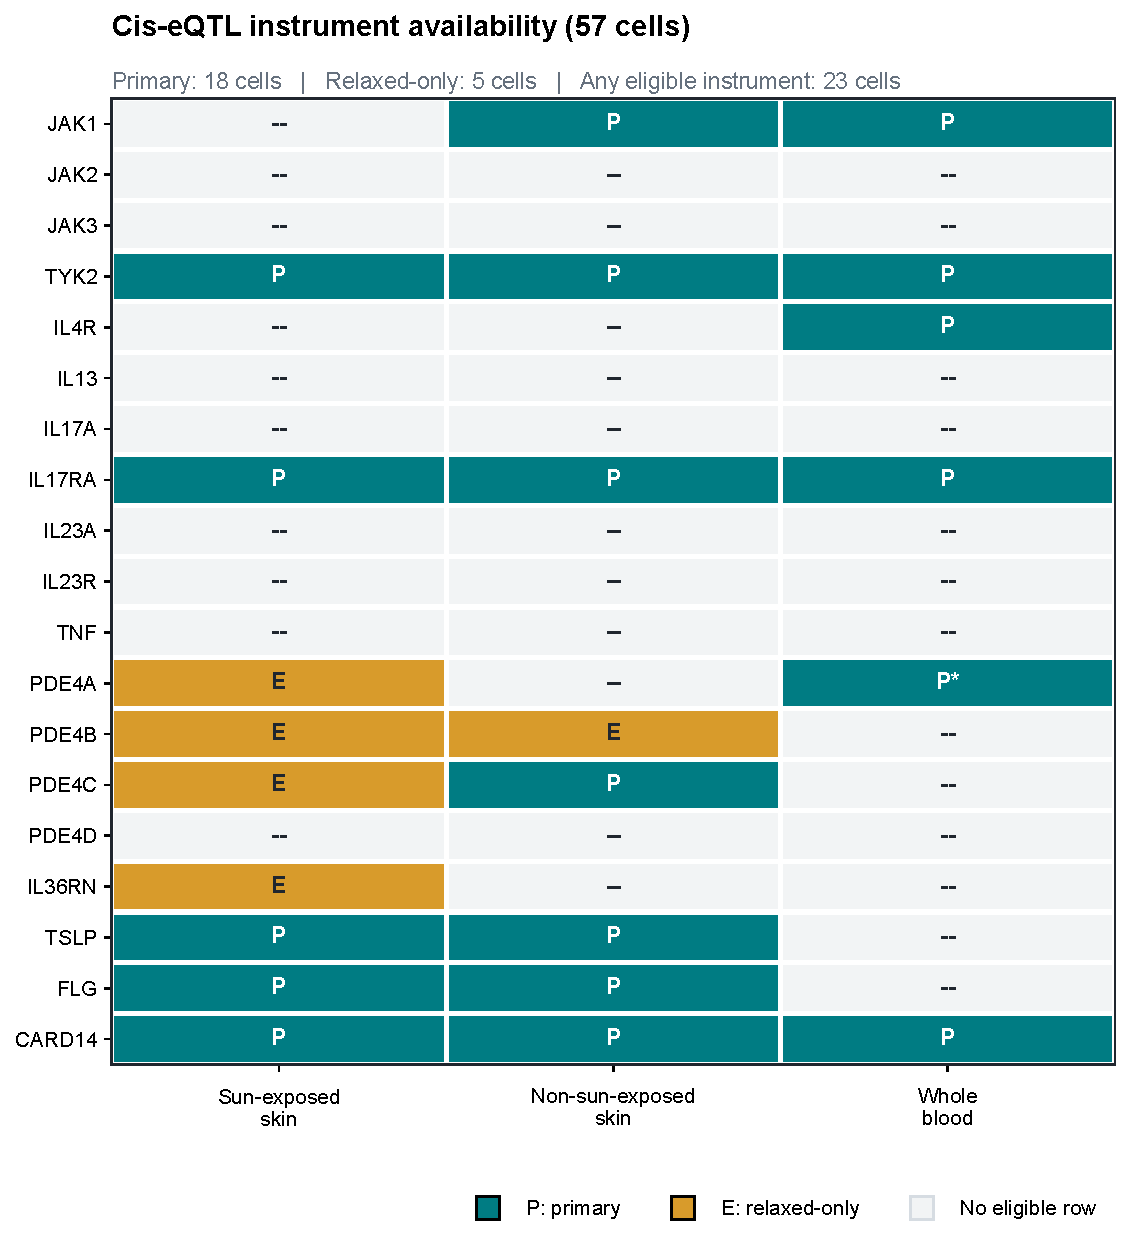
\includegraphics[width=\textwidth,height=0.64\textheight,keepaspectratio]{figure3_instrument_availability_heatmap.pdf}
\caption{Instrument availability across 57 gene--tissue cells. Dark cells denote primary instruments (\textit{p} $<5\times10^{-8}$ and F $>10$), lighter cells denote relaxed-only exploratory instruments (\textit{p} $<10^{-5}$ and F $>10$ in cells lacking a primary instrument), and unfilled cells denote no eligible row in the analyzed GTEx significant-pair file. The asterisk on the PDE4A whole-blood primary cell indicates that the selected variant did not overlap the FinnGen outcomes.}
\label{fig:3}
\end{figure}

\clearpage
\begin{figure}[H]
\centering
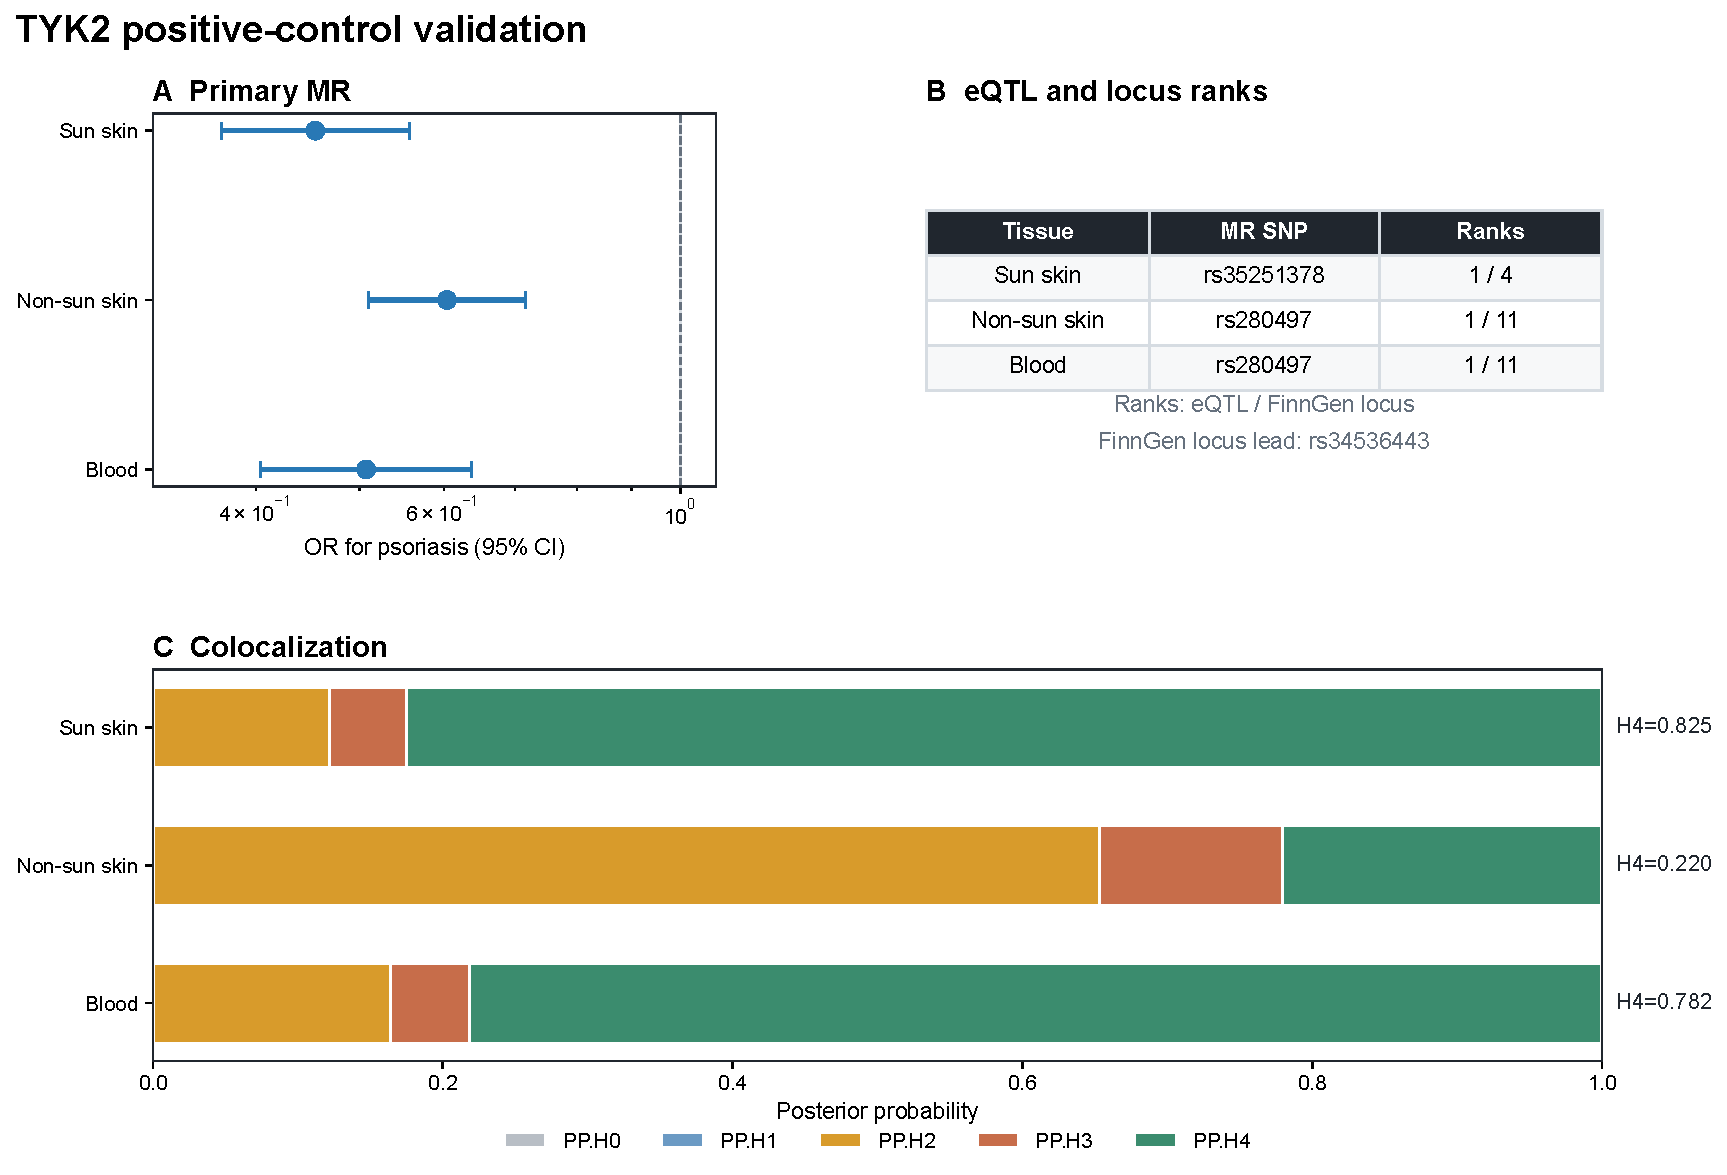
\includegraphics[width=\textwidth,height=0.62\textheight,keepaspectratio]{figure4_tyk2_validation_summary.pdf}
\caption{TYK2 positive-control validation. Panel A summarizes the three primary psoriasis estimates. Panel B shows that rs35251378 and rs280497 were the rank-1 TYK2 eQTLs in their respective tissues and ranked fourth and eleventh, respectively, within the FinnGen TYK2 psoriasis locus, whose lead variant was rs34536443. Panel C shows tissue-resolved colocalization: PP.H4 was 0.825 in sun-exposed skin, 0.782 in whole blood, and 0.220 in non-sun-exposed skin.}
\label{fig:4}
\end{figure}


\end{document}
